\documentclass[]{article}
\usepackage{geometry,tikz,lipsum,amsmath,amssymb,soul,xcolor,cancel,esint}
\tikzset{every picture/.style={line width=0.75pt}} %set default line width to 0.75pt        
\numberwithin{equation}{section}

\NewDocumentCommand{\caja}{ m O{gray!40} O{gray!10} m }{
	\begin{figure}[h]
		\centering
		\begin{tikzpicture}
			\node[anchor=text, text width=\columnwidth-1.2cm, draw, rounded corners, line width=1pt, fill=#3, inner sep=5mm] (big) {\\#4};
			\node[draw, rounded corners, line width=.5pt, fill=#2, anchor=west, xshift=5mm] (small) at (big.north west) {#1};
		\end{tikzpicture}
	\end{figure}
}
\NewDocumentCommand{\indUpDown}{ O{\Lambda} O{\mu} O{\nu} }{
	{#1}^{#2}_{\ #3}
}
\NewDocumentCommand{\indDownUp}{ O{\Lambda} O{\mu} O{\nu} }{
	{#1}_{#2}^{\ #3}
}
\newcommand{\LambdaMuNu}{\indUpDown}
\newcommand{\0}{\textcolor{gray}{0}}
\newcommand{\rbf}{\mathbf{r}}
\newcommand{\ei}{\mathbf{e}_i}
\newcommand{\ej}{\mathbf{e}_j}
\newcommand{\lc}{\epsilon_{ijk}}
\newcommand{\gr}{\nabla}
\newcommand{\di}{\nabla\cdot}
\newcommand{\ro}{\nabla\times}
\newcommand{\la}{\nabla^2}
\newcommand{\xhat}{\hat{\mathbf{x}}}
\newcommand{\yhat}{\hat{\mathbf{y}}}
\newcommand{\zhat}{\hat{\mathbf{z}}}
\newcommand{\rhat}{\hat{\mathbf{r}}}
\newcommand{\that}{\hat{\mathbf{\theta}}}
\newcommand{\phat}{\hat{\mathbf{\varphi}}}
\newcommand{\rhhat}{\hat{\mathbf{\rho}}}
\newcommand{\eo}{\epsilon_0}
\newcommand{\ke}{\frac{1}{4\pi\eo}}
\newcommand{\rv}{\mathbf{r}}
\newcommand{\rdif}{\rv - \rv'}
%opening
\title{Electrodinámica Avanzada}
\author{Simon Fonseca}

\begin{document}
\maketitle

\section{Análisis vectorial}

\subsection{Objetos básicos}
Consideraremos distintos tipos de objetos matemáticos que pueden depender de la posición \(\rbf\) y el tiempo \(t\), los cuales pueden agruparse como:
\begin{enumerate}
	\item \textbf{Campos escalares}: Un valor real para cada punto del espacio
	\begin{equation}
		\phi = \phi(\rbf,t)
		\label{campo_escalar}
	\end{equation}
	\item \textbf{Campos vectoriales}: Un vector para cada punto del espacio
	\begin{equation}
		\mathbf{A} = \mathbf{A}(\rbf,t)
		\label{campo_vectorial}
	\end{equation}
	\item \textbf{Campos tensoriales}: Relaciones multilineales definidas en cada punto del espacio
	\begin{equation}
	D_{ij} = D_{ij}(\rbf,t)
	\label{campo_tensorial}
	\end{equation}
\end{enumerate}

\textbf{Base ortonormal}:
\begin{equation}
	\{\mathbf{e}_1,\mathbf{e}_2,\mathbf{e}_3\} = \{\xhat,\yhat,\zhat\}
	\label{base_ortonormal}
\end{equation}
podemos escribir cualquier vector como
\begin{equation}
	\mathbf{A} = A_i \ei
\end{equation}
bla bla bla \textbf{notación de Einstein}. Las relaciones entre bases ortonormales:
\begin{equation}
	\ei\cdot\ej = \delta_{ij}
\end{equation}
donde \(\delta_{ij}\) es la \textbf{delta de Kronecker}, que cumple que:
\begin{equation}
	\delta_{ij} = \left\lbrace \begin{matrix}
		1,& i = j\\
		0,& i\neq j
	\end{matrix}\right. 
\end{equation}

Tomando:
\begin{equation}
	\partial_i \equiv \dfrac{\partial}{\partial x^i}
\end{equation}
El operador diferencial se define como:
\begin{equation}
	\nabla = \ei\partial_i
\end{equation}
Por lo que también se puede definir la derivada normal en una superficie tal que:
\begin{equation}
	\frac{\partial}{\partial n} = \hat{\mathbf{n}}\cdot\nabla
\end{equation}

\subsection{Operaciones vectoriales}	
Como el espacio es Euclideano (por ahora), no nos preocupamos mucho por los sub y superíndices (cof cof clásica avanzada). Con notación covariante, las operaciones entre vectores en 3 dimensiones:
\begin{table}[h]
	\centering
	\begin{tabular}{c|c}
		\textbf{Operación} & [\texttt{Notación vectorial}] = [\texttt{covariante}] \\
		\hline
		Producto punto & \(\mathbf{A}\cdot\mathbf{B} = A_iB_i\) \\
		\hline
		Producto cruz & \((\mathbf{A}\times\mathbf{B})_i = \lc A_jB_k\) \\
		\hline
		Norma & \(|\mathbf{A}|^2 = \mathbf{A}\cdot\mathbf{A} = A_iA_i\) \\
		\hline
		Gradiente & \(\gr\phi = \ei\partial_i\phi\) \\
		\hline
		Divergencia & \(\di\mathbf{A}=\partial_i A_i\) \\
		\hline
		Rotacional & \(\ro\mathbf{A}=\lc \partial_j A_k\)
	\end{tabular}
\end{table}

\subsection{Identidades vectoriales}
\begin{align}
	\ro(\gr\phi) &= \mathbf{0}\label{idvec1}\\
	\di(\ro\mathbf{A}) &= 0\label{idvec2}\\
	\ro(\ro\mathbf{A}) &= \nabla(\nabla\cdot\mathbf{A})-\nabla^2\mathbf{A}\label{idvec3}\\
	\di(\phi\gr\varphi) &= \phi\la\varphi + \gr\phi\cdot\gr\varphi\label{idvec4}
\end{align}

\subsection{Teoremas integrales}
\subsubsection{Teorema de la divergencia (o Gauss)}
Si \(S(V)\) es la superficie cerrada que delimita el volumen \(V\), entonces
\begin{equation}
	\iiint_V (\di \mathbf{A})dV = \oiint_{S(V)}\mathbf{A}\cdot d\mathbf{S}
	\label{teo_div}
\end{equation}

\subsubsection{Teorema de Stokes}
Si \(S\) es una superficie orientada cuya frontera es la curva cerrada \(C = \partial S\), entonces
\begin{equation}
	\iint_S (\ro\mathbf{A})\cdot d\mathbf{S} = \oint_{C}\mathbf{A}\cdot d\mathbf{r}
	\label{teo_sto}
\end{equation}

\subsubsection{Teorema de Green en el plano}
En dos dimensiones, el teorema de Stokes toma la forma
\begin{equation}
	\iint_R (\partial_x N - \partial_y M)dxdy = \oint_{C}(Mdx + Ndy)
	\label{teo_gre_plano}
\end{equation}
donde \(R\) es la región plana encerrada por \(C\).

\subsubsection{Otra integral útil}
Una identidad adicional que aparece con frecuencia es
\begin{equation}
	\iiint_V (\ro \mathbf{A})dV = \oiint_{S(V)}d\mathbf{S}\times\mathbf{A}
	\label{teo_int}
\end{equation}

\subsection{Coordenadas curvilíneas ortogonales}
Cuando la simetría del problema lo sugiere, conviene abandonar las coordenadas cartesianas y usar 	coordenadas curvilíneas ortogonales \((u_1, u_2, u_3)\). La idea es adaptar el sistema de coordenadas a la 	geometría del problema.

La posición se describe mediante
\begin{equation}
	\mathbf{r} = \mathbf{r}(u_1, u_2, u_3)
\end{equation}
El desplazamiento diferencial es
\begin{equation}
	d\mathbf{r} = \frac{\partial\mathbf{r}}{\partial u_i}du_i
\end{equation}
Definimos los factores de escala \(h_i\) y los vectores locales \(\ei\) por
\begin{equation}
	\begin{matrix}
		\dfrac{\partial\mathbf{r}}{\partial u_i} = h_i\ei, & \mathbf{r} \equiv \dfrac{1}{h_i}\dfrac{\partial\mathbf{r}}{\partial u_i}
	\end{matrix}
\end{equation}
Así,
\begin{equation}
	d\mathbf{r} = h_i du_i \ei
\end{equation}
Y la métrica:
\begin{equation}
	ds^2 = d\mathbf{r}\cdot d\mathbf{r} = g_{ij}du^idu^j
\end{equation}
En un sistema ortogonal (sin términos cruzados),
\begin{equation}
	ds^2 = (h_idu^i)^2
\end{equation}

\subsubsection{Operadores diferenciales en forma general}
Para un campo escalar \(\phi\) y un campo vectorial \(\mathbf{A}\), las expresiones en coordenadas curvilíneas ortogonales son las siguientes:
\begin{enumerate}
	\item \textbf{Gradiente}
	\begin{equation}
		\gr\phi = \sum_{i=1}^{3}\ei\frac{1}{h_i}\frac{\partial\phi}{\partial u_i}
	\end{equation}
	\item \textbf{Divergencia}
	\begin{equation}
		\di\mathbf{A} = \frac{1}{h_1h_2h_3}\left(\sum_{i=1}^{3}\frac{\partial A_i}{\partial u_i}\right) 
	\end{equation}
	\item \textbf{Rotacional}
	\begin{equation}
		\ro\mathbf{A} = \frac{1}{h_1h_2h_3}\begin{vmatrix}
			h_1\mathbf{e}_1 & h_2\mathbf{e}_2 & h_3\mathbf{e}_3\\
			\partial/\partial u_1 & \partial/\partial u_2 & \partial/\partial u_3\\
			h_1A_1 & h_2A_2 & h_3A_3
		\end{vmatrix}
	\end{equation}
	\item \textbf{Laplaciano}
	\begin{equation}
		\la\phi = \frac{1}{h_1h_2h_3}\left[\frac{\partial}{\partial u_i}\left(\frac{u_j u_k}{u_i}\frac{\partial\phi}{\partial u_i}\right) \right]
	\end{equation}
\end{enumerate}

\subsubsection{Coordenadas esféricas}
La transformación entre coordenadas esféricas y cartesianas:
\begin{equation}
	\begin{matrix}
		x = r\sin\theta\cos\varphi,& y = r\sin\theta\sin\varphi,& z = r\cos\theta\\
		r = \sqrt{x^2 + y^2 + z^2},& \theta = \arctan\left(\dfrac{\sqrt{x^2 + y^2}}{z}\right), & \varphi = \arctan\left(\dfrac{y}{x}\right)
	\end{matrix}
\end{equation}
Para vectores ortogonales:
\begin{align}
	\xhat &= \rhat\sin\theta\cos\varphi + \that\cos\theta\cos\varphi - \phat\sin\varphi \\
	\yhat &= \rhat\sin\theta\sin\varphi + \that\cos\theta\sin\varphi + \phat\cos\varphi\\
	\zhat &= \rhat\cos\theta - \that\sin\theta
\end{align}
\begin{align}
	\rhat &= \xhat\sin\theta\cos\varphi + \yhat\sin\theta\sin\varphi + \zhat\cos\theta = \xhat\dfrac{x}{r} + \yhat\dfrac{y}{r} + \zhat\dfrac{z}{r}\\
	\that &= \xhat\cos\theta\cos\varphi + \yhat\cos\theta\sin\varphi - \zhat\sin\theta = \xhat\dfrac{x z}{r\sqrt{x^2+y^2}} + \yhat\dfrac{y z}{r\sqrt{x^2+y^2}} - \zhat\dfrac{\sqrt{x^2+y^2}}{r}\\
	\phat &= - \xhat\sin\varphi + \yhat\cos\varphi = - \xhat\dfrac{y}{\sqrt{x^2+y^2}} + \yhat\dfrac{x}{\sqrt{x^2+y^2}}
\end{align}
La métrica:
\begin{equation}
	ds^2 = dr^2 + r^2\left(d\theta^2 + \sin^2\theta d\varphi^2\right)
\end{equation}
y los factores de escala:
\begin{equation}
	\begin{matrix}
		h_r = 1, & h_\theta = r, & h_\varphi = r\sin\theta
	\end{matrix}
\end{equation}

\subsubsection{Coordenadas cilíndricas}
La transformación entre coordenadas cilíndricas y cartesianas:\footnote{Para ser más exactos, \(\varphi = \) indeterminado, si \(x=y=0\); ; \(\varphi = \frac{\pi}{2}\frac{y}{|y|}\), si \(x=0, y\neq 0\); \(\varphi = \arctan\left(\frac{y}{x}\right)\), si \(x>0\); \(\varphi = \arctan\left(\frac{y}{x}\right) + \pi\), si \(x<0, y\geq0\); \(\varphi = \arctan\left(\frac{y}{x}\right) - \pi\), si \(x<0, y<0\). }
\begin{equation}
	\begin{matrix}
		x = \rho\cos\varphi,& y = \rho\sin\varphi,& z = z\\
		\rho = \sqrt{x^2 + y^2},& \varphi = \arctan\left(\dfrac{y}{x}\right), & z = z
	\end{matrix}
\end{equation}
Para vectores ortogonales:
\begin{align}
	\xhat &= \rhhat\cos\varphi - \phat\sin\varphi \\
	\yhat &= \rhhat\sin\varphi + \that\cos\varphi \\
	\zhat &= \zhat
\end{align}
\begin{align}
	\rhhat &= \xhat\cos\varphi + \yhat\sin\varphi = \xhat\dfrac{x}{\sqrt{x^2+y^2}} + \yhat\dfrac{y}{\sqrt{x^2+y^2}}\\
	\phat  &= -\xhat\sin\varphi + \yhat\cos\varphi = -\xhat\dfrac{y}{\sqrt{x^2+y^2}} + \yhat\dfrac{x}{\sqrt{x^2+y^2}}\\
	\zhat  &= \zhat
\end{align}
La métrica:
\begin{equation}
	ds^2 = d\rho^2 + \rho^2 d\varphi^2 + dz^2
\end{equation}
y los factores de escala:
\begin{equation}
	\begin{matrix}
		h_\rho = 1, & h_\varphi = \rho, & h_z = 1
	\end{matrix}
\end{equation}
	
\section{Electrostática}
\subsection{Ley de Coulomb y campo eléctrico}
La \textbf{ley de Coulomb} define la interacción entre cargas puntuales:
\begin{equation}
	\mathbf{F}_{12} = \ke\frac{q_1q_2}{|\mathbf{r}_1 - \mathbf{r}_2|^3}(\mathbf{r}_1 - \mathbf{r}_2)
\end{equation}

Si definimos el campo eléctrico como fuerza eléctrica por unidad de carga ejercida por una carga puntual \(q\) en posición \(\mathbf{r}_0\):
\begin{equation}
	\mathbf{E}(\mathbf{r}) = \ke q\frac{\mathbf{r} - \mathbf{r}_0}{|\mathbf{r} - \mathbf{r}_0|^3}
\end{equation}

Para varias cargas discretas \(q_i\) en posiciones \(\mathbf{r}_i\):
\begin{equation}
	\mathbf{E}(\mathbf{r}) = \ke \sum_{i}q_i\frac{\mathbf{r} - \mathbf{r}_i}{|\mathbf{r} - \mathbf{r}_i|^3}
\end{equation}

En el caso de densidades de carga lineal (\(\lambda\)), superficial (\(\sigma\)) y volumétrica (\(\rho\)), tendremos las expresiones:
\begin{align}
	\mathbf{E}(\mathbf{r}) &= \ke \int dl'\lambda(\mathbf{r}')\frac{\mathbf{r} - \mathbf{r}'}{|\mathbf{r} - \mathbf{r}'|^3}\\
	\mathbf{E}(\mathbf{r}) &= \ke \iint da'\sigma(\mathbf{r}')\frac{\mathbf{r} - \mathbf{r}'}{|\mathbf{r} - \mathbf{r}'|^3}\\
	\mathbf{E}(\mathbf{r}) &= \ke \iiint d^3r'\rho(\mathbf{r}')\frac{\mathbf{r} - \mathbf{r}'}{|\mathbf{r} - \mathbf{r}'|^3}
\end{align}

\subsection{Ley de Gauss}
La \textbf{ley de Gauss} afirma que para cualquier superficie cerrada \(S\)
\begin{equation}
	\oiint_{S} \mathbf{E}\cdot d\mathbf{S} = \frac{Q_{\text{enc}}}{\eo}
\end{equation}
donde \(Q_{\text{enc}}\) es la carga total encerrada. Si la carga es continua,
\begin{equation*}
	Q_{\text{enc}} = \iiint_{V(S)} \rho(\mathbf{r}) d^3r
\end{equation*}

En forma diferencial:
\begin{equation}
	\di\mathbf{E} = \frac{\rho}{\eo}
\end{equation}

\subsection{Potencial electrostático}
La fuerza y, por ende, el campo eléctrico son campos conservativos, por lo que podemos escribir un potencial escalar \(\Phi(\mathbf{r})\) tal que:
\begin{align}
	\mathbf{E} &= -\gr\Phi\\
	\Rightarrow \Delta\Phi &= -\int_{A}^{B} \mathbf{E}\cdot d\mathbf{l}
\end{align}

Si fijamos el potencial en el infinito como nulo \(\Phi(\infty) = 0\), tendremos:
\begin{equation}
	\Phi(\mathbf{r}) = \ke\frac{q}{r}
\end{equation}

Como \(\mathbf{E}\) es conservativo, también tendremos que su rotacional es nulo:
\begin{align}
	\ro\mathbf{E} &= 0\\
	\oint_C\mathbf{E}\cdot d\mathbf{l} &= 0
\end{align}

Y la \textbf{energía potencial} para cargas discretas:
\begin{equation}
	U=\frac{1}{2}\sum_{i}q_i\Phi(\mathbf{r}_i)
\end{equation}
y para una distribución continua:
\begin{equation}
	U = \frac{1}{2}\int\rho(\mathbf{r})\Phi(\mathbf{r})d^3r
\end{equation}

\subsection{Condiciones de borde}
\subsubsection{Salto de la componente normal del campo}
Sea una interfaz con densidad superficial de carga libre \(\sigma\)
\begin{equation}
	(\mathbf{E}_2 - \mathbf{E}_1)\cdot\hat{\mathbf{n}} = \frac{\sigma}{\eo}
\end{equation}
donde \(\hat{\mathbf{n}}\) apunta de la región 1 a la región 2. 

\subsubsection{Continuidad de la componente tangencial}
Como en electrostática se cumple \(\ro \mathbf{E} = 0\), la circulación sobre un contorno infinitesimal que cruza la frontera da
\begin{equation}
	\hat{\mathbf{n}}\times(\mathbf{E}_2 - \mathbf{E}_1) = 0
\end{equation}
La componente tangencial del campo es, por tanto, continua. 

\subsubsection{Potencial en la frontera}
Puesto que \(\mathbf{E} = -\gr\Phi\), la continuidad de la componente tangencial de \(\mathbf{E}\) implica la continuidad del potencial en una superficie ordinaria
\begin{equation}
	\Phi_1 = \Phi_2
\end{equation}
Sin embargo, su derivada normal puede ser discontinua. En particular
\begin{equation}
	\left. \frac{\partial\Phi_2}{\partial n} - \frac{\partial\Phi_1}{\partial n}\right|_S = - \frac{\sigma}{\eo}
\end{equation}

\subsubsection{Conductores en equilibrio electrostático}
En un conductor ideal en equilibrio electrostático se cumplen las siguientes propiedades:
\begin{enumerate}
	\item el campo en el interior del conductor es nulo;
	\item el potencial es constante en todo el conductor;
	\item la superficie del conductor es una superficie equipotencial;
	\item la componente tangencial del campo sobre la superficie es cero;
	\item la carga libre reside sobre la superficie.
\end{enumerate}

\subsection{Ecuaciones de Poisson y Laplace}
\textbf{Ecuación de Poisson}:
\begin{equation}
	\la\Phi = - \frac{\rho}{\eo}
\end{equation}
En regiones libres de carga (\(\rho=0\)) tenemos la \textbf{ecuación de Laplace}:
\begin{equation}
	\la\Phi = 0
\end{equation}
Las soluciones de Laplace se llaman funciones armónicas.

La solución de la ecuación de Poisson en el espacio libre:
\begin{equation}
	\Phi(\mathbf{r}) = \ke\int d^3\mathbf{r}'\frac{\rho(\mathbf{r}')}{|\mathbf{r}-\mathbf{r}'|}
\end{equation}

\subsection{Identidades y funciones de Green}
Partiendo del teorema de la divergencia (ecuación \ref{teo_div}):
\begin{equation*}
	\int_{V}(\di\mathbf{A})dV = \oint_{S}(\mathbf{A}\cdot\hat{\mathbf{n}})dS
\end{equation*}
Y tomando
\begin{equation*}
	\mathbf{A} = \phi\gr\varphi,
\end{equation*}
donde \(\phi,\varphi\) son funciones escalares. Entonces, usando la ecuación\ref{idvec4}, llegamos a la \textbf{primera identidad de Green}:
\begin{equation}
	\int_{V}(\phi\la\varphi + \gr\phi\cdot\gr\varphi)dV = \oint_{S}\phi\frac{\partial\varphi}{\partial n}dS
	\label{1_id_green}
\end{equation}
Si elegimos \(\phi=\varphi=u\)
\begin{equation}
	\int_{V}(u\la u + |\gr u|^2dV = \oint_{S}u\frac{\partial u}{\partial n}dS
\end{equation}

Si ahora intercambiamos \(\phi\leftrightarrow\varphi\) y restamos la expresión \ref{1_id_green} con esta, obtenemos la  \textbf{segunda identidad de Green}:
\begin{equation}
	\int_{V}(\phi\la\varphi + \varphi\la\phi)dV = \oint_{S}\left(\phi\frac{\partial\varphi}{\partial n} - \varphi\frac{\partial\phi}{\partial n}\right)dS
	\label{2_id_green}
\end{equation}

Buscamos una función \(G(\mathbf{r}, \mathbf{r}')\) tal que, considerada como función de \(\mathbf{r}'\) para \(\mathbf{r}\) fijo, satisfaga
\begin{equation}
	\nabla'^2 G(\mathbf{r}, \mathbf{r}') = -4\pi\delta(\rdif)
\end{equation}
en el volumen de interés, junto con condiciones de borde adecuadas en la superficie \(S\). El símbolo \(\nabla'^2\) indica que el laplaciano actúa sobre la variable fuente \(\rv'\). En espacio libre la elección más simple es
\begin{equation}
	G_0(\rv,\rv') = \frac{1}{|\rdif|}
\end{equation}

Partiendo de la segunda identidad de Green y considerando:
\begin{equation*}
	\begin{matrix}
		\phi(\rv') = \Phi(\rv'),& \varphi(\rv') = G(\rv,\rv')
	\end{matrix}
\end{equation*}
\begin{equation*}
	\Rightarrow \int_{V}(\Phi\la G + G\la\Phi)dV = \oint_{S}\left(\Phi\frac{\partial G}{\partial n'} -  G\frac{\partial\Phi}{\partial n'}\right)dS'
\end{equation*}
Usando ahora
\begin{equation*}
	\begin{matrix}
		\nabla'^2 G(\mathbf{r}, \mathbf{r}') = -4\pi\delta(\rdif),& \la\Phi(\rv') = - \dfrac{\rho(\rv')}{\eo}
	\end{matrix}
\end{equation*}
obtenemos
\begin{equation*}
	\Rightarrow -4\pi\Phi + \frac{1}{\eo}\int_{V}G\rho d^3r' = \oint_{S}\left(\Phi\frac{\partial G}{\partial n'} -  G\frac{\partial\Phi}{\partial n'}\right)dS'
\end{equation*}
reordenando:
\begin{equation}
	\Phi(\rv) = \frac{1}{4\pi\eo}\int_{V}G\rho d^3r' + \frac{1}{4\pi}\oint_{S}\left( G\frac{\partial\Phi}{\partial n'} - \Phi\frac{\partial G}{\partial n'} \right)dS'
	\label{poisson_sol_green}
\end{equation}
Ésta es la fórmula general de representación para el potencial. Debe leerse con cuidado. El primer término contiene la contribución del volumen; el segundo, la contribución de la superficie. La elección concreta de \(G\) permite que uno de los términos de borde se simplifique dependiendo del tipo de condición de borde impuesta.

Cuando \(\rho = 0\), la ecuación de Poisson se reduce a la de Laplace y la fórmula general queda
\begin{equation}
	\Phi(\rv) = \frac{1}{4\pi}\oint_{S}\left( G\frac{\partial\Phi}{\partial n'} - \Phi\frac{\partial G}{\partial n'} \right)dS'
	\label{laplace_sol_green}
\end{equation}

Si tenemos un potencial conocido en la frontera (como en el caso cuando la superficie es conductora y se conoce el potencial sobre ella), conviene elegir una función de Green de Dirichlet que satisfaga
\begin{equation*}
	\begin{matrix}
		G_D(\rv,\rv') = 0,& \rv'\in S
	\end{matrix}
\end{equation*}
Entonces el primer término de superficie en la ecuación \ref{poisson_sol_green} desaparece y queda
\begin{equation}
	\Phi(\rv) = \frac{1}{4\pi\eo}\int_{V}G_D\rho d^3r' - \frac{1}{4\pi}\oint_{S}\Phi\frac{\partial G_D}{\partial n'} dS'
\end{equation}

Bajo hipótesis estándar y para condiciones de borde apropiadas, la función de Green satisface una propiedad de reciprocidad:
\begin{equation}
	G(\rv, \rv') = G(\rv', \rv)
\end{equation}

La función de Green puede interpretarse como el potencial en el punto \(\rv\) producido por una carga puntual unitaria situada en \(\rv'\), en presencia de las fronteras del problema. Incorpora simultáneamente la ley local de interacción (laplaciano en volumen) y la geometría global de la región (condiciones de borde).

\subsection{Método de las imágenes}
El método de imágenes puede entenderse como una manera ingeniosa de construir funciones de Green en ciertas geometrías simples. En lugar de resolver el problema de contorno de manera abstracta, se reemplaza la presencia de la frontera por cargas ficticias situadas fuera de la región física.

\subsubsection{Ejemplo 1}
Considérese una carga puntual \(q\) en el punto \((0, 0, a)\), con \(a > 0\), frente a un plano conductor infinito ubicado en \(z = 0\) y conectado a tierra. En la región \(z > 0\) se desea resolver
\begin{equation*}
	\begin{matrix}
		\la\Phi = -\dfrac{q}{\eo}\delta(x)\delta(y)\delta(z-a),& \Phi(x,y,0) = 0
	\end{matrix}
\end{equation*}
La solución se obtiene colocando una carga imagen \(-q\) en \((0, 0, -a)\). El potencial para \(z > 0\) es
\begin{equation*}
	\Phi(x,y,z>0) = \ke\left[\frac{q}{\sqrt{x^2+y^2+(z-a)^2}} - \frac{q}{\sqrt{x^2+y^2+(z+a)^2}} \right] 
\end{equation*}
\begin{figure}[h!]
	\centering
	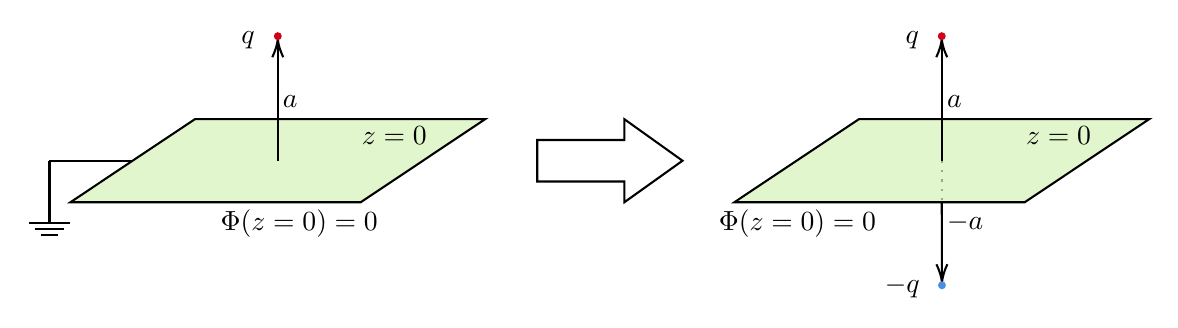
\begin{tikzpicture}[x=0.75pt,y=0.75pt,yscale=-1,xscale=1]
		%uncomment if require: \path (0,300); %set diagram left start at 0, and has height of 300
		
		%Shape: Parallelogram [id:dp7825764686002114] 
		\draw  [fill={rgb, 255:red, 184; green, 233; blue, 134 }  ,fill opacity=0.42 ] (90.04,90) -- (229.9,90) -- (169.96,130) -- (30.1,130) -- cycle ;
		%Straight Lines [id:da1937112930016054] 
		\draw    (130,110) -- (130,53.38) ;
		\draw [shift={(130,51.38)}, rotate = 90] [color={rgb, 255:red, 0; green, 0; blue, 0 }  ][line width=0.75]    (8.74,-2.63) .. controls (5.56,-1.12) and (2.65,-0.24) .. (0,0) .. controls (2.65,0.24) and (5.56,1.12) .. (8.74,2.63)   ;
		%Shape: Circle [id:dp3196027884747259] 
		\draw  [color={rgb, 255:red, 208; green, 2; blue, 27 }  ,draw opacity=1 ][fill={rgb, 255:red, 208; green, 2; blue, 27 }  ,fill opacity=1 ][line width=0.75]  (128.63,50) .. controls (128.63,49.24) and (129.24,48.63) .. (130,48.63) .. controls (130.76,48.63) and (131.38,49.24) .. (131.38,50) .. controls (131.38,50.76) and (130.76,51.38) .. (130,51.38) .. controls (129.24,51.38) and (128.63,50.76) .. (128.63,50) -- cycle ;
		%Straight Lines [id:da7565707012841785] 
		\draw [color={rgb, 255:red, 128; green, 128; blue, 128 }  ,draw opacity=1 ] [dash pattern={on 0.84pt off 2.51pt}]  (449.9,110) -- (449.9,130) ;
		%Straight Lines [id:da6716488010045845] 
		\draw    (449.9,130) -- (449.99,166.63) ;
		\draw [shift={(450,168.63)}, rotate = 269.85] [color={rgb, 255:red, 0; green, 0; blue, 0 }  ][line width=0.75]    (8.74,-2.63) .. controls (5.56,-1.12) and (2.65,-0.24) .. (0,0) .. controls (2.65,0.24) and (5.56,1.12) .. (8.74,2.63)   ;
		%Shape: Circle [id:dp03421088388923921] 
		\draw  [color={rgb, 255:red, 74; green, 144; blue, 226 }  ,draw opacity=1 ][fill={rgb, 255:red, 74; green, 144; blue, 226 }  ,fill opacity=1 ][line width=0.75]  (451.38,170) .. controls (451.38,170.76) and (450.76,171.38) .. (450,171.38) .. controls (449.24,171.38) and (448.63,170.76) .. (448.63,170) .. controls (448.63,169.24) and (449.24,168.63) .. (450,168.63) .. controls (450.76,168.63) and (451.38,169.24) .. (451.38,170) -- cycle ;
		%Shape: Parallelogram [id:dp8452425109380757] 
		\draw  [fill={rgb, 255:red, 184; green, 233; blue, 134 }  ,fill opacity=0.42 ] (409.94,90) -- (549.8,90) -- (489.86,130) -- (350,130) -- cycle ;
		%Straight Lines [id:da48227188013868283] 
		\draw    (449.9,110) -- (449.9,53.38) ;
		\draw [shift={(449.9,51.38)}, rotate = 90] [color={rgb, 255:red, 0; green, 0; blue, 0 }  ][line width=0.75]    (8.74,-2.63) .. controls (5.56,-1.12) and (2.65,-0.24) .. (0,0) .. controls (2.65,0.24) and (5.56,1.12) .. (8.74,2.63)   ;
		%Shape: Circle [id:dp5576822087853077] 
		\draw  [color={rgb, 255:red, 208; green, 2; blue, 27 }  ,draw opacity=1 ][fill={rgb, 255:red, 208; green, 2; blue, 27 }  ,fill opacity=1 ][line width=0.75]  (448.53,50) .. controls (448.53,49.24) and (449.14,48.63) .. (449.9,48.63) .. controls (450.66,48.63) and (451.28,49.24) .. (451.28,50) .. controls (451.28,50.76) and (450.66,51.38) .. (449.9,51.38) .. controls (449.14,51.38) and (448.53,50.76) .. (448.53,50) -- cycle ;
		%Straight Lines [id:da335348609873486] 
		\draw    (60,110) -- (20,110) ;
		%Straight Lines [id:da15282303022062482] 
		\draw    (20,110) -- (20,140) ;
		%Straight Lines [id:da062370163799205236] 
		\draw    (10,140) -- (30,140) ;
		%Straight Lines [id:da8144980721938546] 
		\draw    (12.86,143) -- (27.14,143) ;
		%Straight Lines [id:da400864248266933] 
		\draw    (15.71,146) -- (24.29,146) ;
		
		%Right Arrow [id:dp12082924455938926] 
		\draw   (255,100) -- (297,100) -- (297,90) -- (325,110) -- (297,130) -- (297,120) -- (255,120) -- cycle ;
		
		% Text Node
		\draw (111,46.4) node [anchor=north west][inner sep=0.75pt]    {$q$};
		% Text Node
		\draw (131,77) node [anchor=north west][inner sep=0.75pt]   [align=left] {$\displaystyle a$};
		% Text Node
		\draw (101,132) node [anchor=north west][inner sep=0.75pt]   [align=left] {$\displaystyle \Phi ( z=0) =0$};
		% Text Node
		\draw (169,92) node [anchor=north west][inner sep=0.75pt]   [align=left] {$\displaystyle z=0$};
		% Text Node
		\draw (431,46.4) node [anchor=north west][inner sep=0.75pt]    {$q$};
		% Text Node
		\draw (451,77) node [anchor=north west][inner sep=0.75pt]   [align=left] {$\displaystyle a$};
		% Text Node
		\draw (341,132) node [anchor=north west][inner sep=0.75pt]   [align=left] {$\displaystyle \Phi ( z=0) =0$};
		% Text Node
		\draw (489,92) node [anchor=north west][inner sep=0.75pt]   [align=left] {$\displaystyle z=0$};
		% Text Node
		\draw (421,164) node [anchor=north west][inner sep=0.75pt]   [align=left] {$\displaystyle -q$};
		% Text Node
		\draw (451,134) node [anchor=north west][inner sep=0.75pt]   [align=left] {$\displaystyle -a$};	
	\end{tikzpicture}
\end{figure}

\subsubsection{Ejemplo 2}
Intentemos resolver el caso de una esfera conductora conectada a tierra de radio \(a\) y una carga \(q\) a una distancia \(\mathbf{x}\) del centro. Por simetría la carga virtual \(q'\) debe ubicarse dentro de la esfera, en la dirección de descrita por \(\mathbf{x}\). Es decir, buscamos un potencial:
\begin{equation*}
	\Phi(\mathbf{r}) = \ke\frac{q}{|\rv - \mathbf{x}|} + \ke\frac{q'}{|\rv - \mathbf{x}'|}
\end{equation*}
tal que
\begin{equation*}
	\Phi(|\rv|=a)=0
\end{equation*}

\begin{figure}[h!]
	\centering
	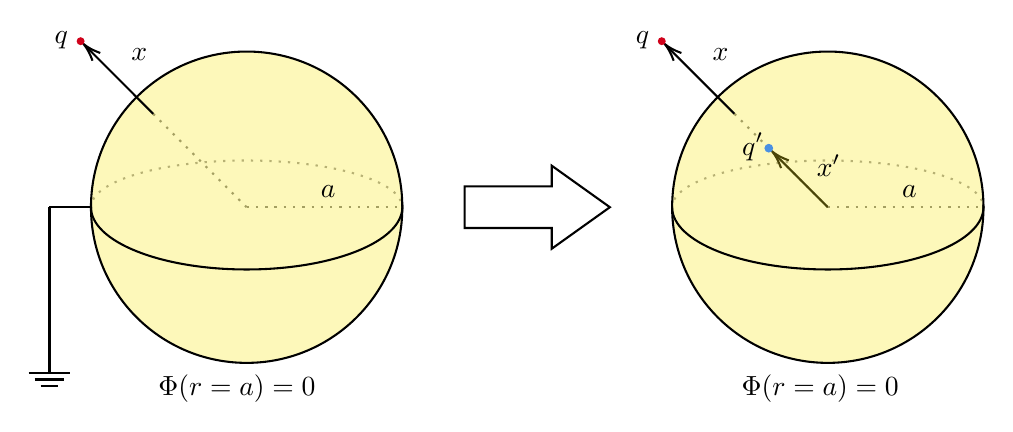
\begin{tikzpicture}[x=0.75pt,y=0.75pt,yscale=-1,xscale=1]
		%uncomment if require: \path (0,300); %set diagram left start at 0, and has height of 300
		
		%Shape: Arc [id:dp7018042493744993] 
		\draw  [draw opacity=0][dash pattern={on 0.84pt off 2.51pt}] (489.88,91.31) .. controls (489.96,90.87) and (490,90.44) .. (490,90) .. controls (490,77.57) and (456.42,67.5) .. (415,67.5) .. controls (373.58,67.5) and (340,77.57) .. (340,90) -- (415,90) -- cycle ; \draw  [color={rgb, 255:red, 155; green, 155; blue, 155 }  ,draw opacity=1 ][dash pattern={on 0.84pt off 2.51pt}] (489.88,91.31) .. controls (489.96,90.87) and (490,90.44) .. (490,90) .. controls (490,77.57) and (456.42,67.5) .. (415,67.5) .. controls (373.58,67.5) and (340,77.57) .. (340,90) ;  
		%Straight Lines [id:da6968020466826599] 
		\draw [color={rgb, 255:red, 128; green, 128; blue, 128 }  ,draw opacity=1 ] [dash pattern={on 0.84pt off 2.51pt}]  (370,45) -- (415,90) ;
		%Straight Lines [id:da3169038390579897] 
		\draw    (415,90) -- (389.59,64.53) ;
		\draw [shift={(388.18,63.12)}, rotate = 45.07] [color={rgb, 255:red, 0; green, 0; blue, 0 }  ][line width=0.75]    (8.74,-2.63) .. controls (5.56,-1.12) and (2.65,-0.24) .. (0,0) .. controls (2.65,0.24) and (5.56,1.12) .. (8.74,2.63)   ;
		%Straight Lines [id:da5314397149547201] 
		\draw    (60,90) -- (40,90) ;
		%Straight Lines [id:da5046521692751513] 
		\draw    (40,90) -- (40,170) ;
		%Straight Lines [id:da31852283803689785] 
		\draw    (30,170) -- (50,170) ;
		%Straight Lines [id:da8621977570733834] 
		\draw    (32.86,173) -- (47.14,173) ;
		%Straight Lines [id:da09358053897737806] 
		\draw    (35.71,176) -- (44.29,176) ;
		
		%Right Arrow [id:dp7292995571276311] 
		\draw   (240,80) -- (282,80) -- (282,70) -- (310,90) -- (282,110) -- (282,100) -- (240,100) -- cycle ;
		%Straight Lines [id:da6796615124546492] 
		\draw [color={rgb, 255:red, 128; green, 128; blue, 128 }  ,draw opacity=1 ] [dash pattern={on 0.84pt off 2.51pt}]  (415,90) -- (416.39,90) -- (490,90) ;
		%Shape: Circle [id:dp022021139273155077] 
		\draw  [fill={rgb, 255:red, 248; green, 231; blue, 28 }  ,fill opacity=0.3 ] (340,90) .. controls (340,48.58) and (373.58,15) .. (415,15) .. controls (456.42,15) and (490,48.58) .. (490,90) .. controls (490,131.42) and (456.42,165) .. (415,165) .. controls (373.58,165) and (340,131.42) .. (340,90) -- cycle ;
		%Shape: Arc [id:dp09338257926922833] 
		\draw  [draw opacity=0] (489.93,88.69) .. controls (489.98,89.13) and (490,89.56) .. (490,90) .. controls (490,106.57) and (456.42,120) .. (415,120) .. controls (373.58,120) and (340,106.57) .. (340,90) -- (415,90) -- cycle ; \draw  [color={rgb, 255:red, 0; green, 0; blue, 0 }  ,draw opacity=1 ] (489.93,88.69) .. controls (489.98,89.13) and (490,89.56) .. (490,90) .. controls (490,106.57) and (456.42,120) .. (415,120) .. controls (373.58,120) and (340,106.57) .. (340,90) ;  
		%Straight Lines [id:da008691646505346706] 
		\draw    (370,45) -- (337.83,12.78) ;
		\draw [shift={(336.42,11.37)}, rotate = 45.05] [color={rgb, 255:red, 0; green, 0; blue, 0 }  ][line width=0.75]    (8.74,-2.63) .. controls (5.56,-1.12) and (2.65,-0.24) .. (0,0) .. controls (2.65,0.24) and (5.56,1.12) .. (8.74,2.63)   ;
		%Shape: Circle [id:dp23043596762466823] 
		\draw  [color={rgb, 255:red, 208; green, 2; blue, 27 }  ,draw opacity=1 ][fill={rgb, 255:red, 208; green, 2; blue, 27 }  ,fill opacity=1 ][line width=0.75]  (333.63,10) .. controls (333.63,9.24) and (334.24,8.63) .. (335,8.63) .. controls (335.76,8.63) and (336.38,9.24) .. (336.38,10) .. controls (336.38,10.76) and (335.76,11.38) .. (335,11.38) .. controls (334.24,11.38) and (333.63,10.76) .. (333.63,10) -- cycle ;
		%Shape: Ellipse [id:dp3823465417845865] 
		\draw  [color={rgb, 255:red, 74; green, 144; blue, 226 }  ,draw opacity=1 ][fill={rgb, 255:red, 74; green, 144; blue, 226 }  ,fill opacity=1 ][line width=0.75]  (385,61.56) .. controls (385,60.7) and (385.7,60) .. (386.56,60) .. controls (387.43,60) and (388.13,60.7) .. (388.13,61.56) .. controls (388.13,62.43) and (387.43,63.13) .. (386.56,63.13) .. controls (385.7,63.13) and (385,62.43) .. (385,61.56) -- cycle ;
		%Shape: Arc [id:dp9031009591798822] 
		\draw  [draw opacity=0][dash pattern={on 0.84pt off 2.51pt}] (209.88,91.31) .. controls (209.96,90.87) and (210,90.44) .. (210,90) .. controls (210,77.57) and (176.42,67.5) .. (135,67.5) .. controls (93.58,67.5) and (60,77.57) .. (60,90) -- (135,90) -- cycle ; \draw  [color={rgb, 255:red, 155; green, 155; blue, 155 }  ,draw opacity=1 ][dash pattern={on 0.84pt off 2.51pt}] (209.88,91.31) .. controls (209.96,90.87) and (210,90.44) .. (210,90) .. controls (210,77.57) and (176.42,67.5) .. (135,67.5) .. controls (93.58,67.5) and (60,77.57) .. (60,90) ;  
		%Straight Lines [id:da8813689857714082] 
		\draw [color={rgb, 255:red, 128; green, 128; blue, 128 }  ,draw opacity=1 ] [dash pattern={on 0.84pt off 2.51pt}]  (90,45) -- (135,90) ;
		%Straight Lines [id:da8967443598072239] 
		\draw [color={rgb, 255:red, 128; green, 128; blue, 128 }  ,draw opacity=1 ] [dash pattern={on 0.84pt off 2.51pt}]  (135,90) -- (136.39,90) -- (210,90) ;
		%Shape: Circle [id:dp9868405435875616] 
		\draw  [fill={rgb, 255:red, 248; green, 231; blue, 28 }  ,fill opacity=0.3 ] (60,90) .. controls (60,48.58) and (93.58,15) .. (135,15) .. controls (176.42,15) and (210,48.58) .. (210,90) .. controls (210,131.42) and (176.42,165) .. (135,165) .. controls (93.58,165) and (60,131.42) .. (60,90) -- cycle ;
		%Shape: Arc [id:dp17367635350094546] 
		\draw  [draw opacity=0] (209.93,88.69) .. controls (209.98,89.13) and (210,89.56) .. (210,90) .. controls (210,106.57) and (176.42,120) .. (135,120) .. controls (93.58,120) and (60,106.57) .. (60,90) -- (135,90) -- cycle ; \draw  [color={rgb, 255:red, 0; green, 0; blue, 0 }  ,draw opacity=1 ] (209.93,88.69) .. controls (209.98,89.13) and (210,89.56) .. (210,90) .. controls (210,106.57) and (176.42,120) .. (135,120) .. controls (93.58,120) and (60,106.57) .. (60,90) ;  
		%Straight Lines [id:da7140725276637453] 
		\draw    (90,45) -- (57.83,12.78) ;
		\draw [shift={(56.42,11.37)}, rotate = 45.05] [color={rgb, 255:red, 0; green, 0; blue, 0 }  ][line width=0.75]    (8.74,-2.63) .. controls (5.56,-1.12) and (2.65,-0.24) .. (0,0) .. controls (2.65,0.24) and (5.56,1.12) .. (8.74,2.63)   ;
		%Shape: Circle [id:dp8718588045019053] 
		\draw  [color={rgb, 255:red, 208; green, 2; blue, 27 }  ,draw opacity=1 ][fill={rgb, 255:red, 208; green, 2; blue, 27 }  ,fill opacity=1 ][line width=0.75]  (53.63,10) .. controls (53.63,9.24) and (54.24,8.63) .. (55,8.63) .. controls (55.76,8.63) and (56.38,9.24) .. (56.38,10) .. controls (56.38,10.76) and (55.76,11.38) .. (55,11.38) .. controls (54.24,11.38) and (53.63,10.76) .. (53.63,10) -- cycle ;
		
		% Text Node
		\draw (91,169) node [anchor=north west][inner sep=0.75pt]   [align=left] {$\displaystyle \Phi ( r=a) =0$};
		% Text Node
		\draw (372,169) node [anchor=north west][inner sep=0.75pt]   [align=left] {$\displaystyle \Phi ( r=a) =0$};
		% Text Node
		\draw (449.25,78.25) node [anchor=north west][inner sep=0.75pt]   [align=left] {$\displaystyle a$};
		% Text Node
		\draw (321,4) node [anchor=north west][inner sep=0.75pt]   [align=left] {$\displaystyle q$};
		% Text Node
		\draw (358,12) node [anchor=north west][inner sep=0.75pt]   [align=left] {$\displaystyle x$};
		% Text Node
		\draw (372.25,52.75) node [anchor=north west][inner sep=0.75pt]   [align=left] {$\displaystyle q'$};
		% Text Node
		\draw (408.25,63.25) node [anchor=north west][inner sep=0.75pt]   [align=left] {$\displaystyle x'$};
		% Text Node
		\draw (169.25,78.25) node [anchor=north west][inner sep=0.75pt]   [align=left] {$\displaystyle a$};
		% Text Node
		\draw (41,4) node [anchor=north west][inner sep=0.75pt]   [align=left] {$\displaystyle q$};
		% Text Node
		\draw (78,12) node [anchor=north west][inner sep=0.75pt]   [align=left] {$\displaystyle x$};
	\end{tikzpicture}
\end{figure}

Desarrollando,
\begin{align*}
	\Phi(\mathbf{r}) &= \ke\frac{q}{|r\rhat - x\xhat|} + \ke\frac{q'}{\left|r\rhat - x'\xhat\right|}\\
	\Rightarrow\Phi(\mathbf{r}) &= \ke\frac{q}{r\left|\rhat - \dfrac{x}{r}\xhat\right|} + \ke\frac{q'}{x'\left|\dfrac{r}{x'}\rhat - \xhat\right|}\\
	\Rightarrow\Phi(\mathbf{r} = a) &= \ke\frac{q/a}{\left|\rhat - \dfrac{x}{a}\xhat\right|} + \ke\frac{q'/x'}{\left|\xhat - \dfrac{a}{x'}\rhat\right|} = 0
\end{align*}
Recordando que la magnitud de la suma de dos vectores es:
\begin{align}
	|A\hat{\mathbf{a}} + B\hat{\mathbf{b}}| &= \sqrt{A^2\hat{\mathbf{a}}\cdot\hat{\mathbf{a}} - 2AB\hat{\mathbf{a}}\cdot\hat{\mathbf{b}} + B^2\hat{\mathbf{b}}\cdot\hat{\mathbf{b}}}\nonumber\\
	|A\hat{\mathbf{a}} + B\hat{\mathbf{b}}| &= \sqrt{A + B + 2AB\hat{\mathbf{a}}\cdot\hat{\mathbf{b}}}\\
	\Rightarrow |A\hat{\mathbf{a}} + B\hat{\mathbf{b}}| &= |B\hat{\mathbf{a}} + A\hat{\mathbf{b}}|
\end{align}
Por lo que podemos identificar que
\begin{equation*}
	\begin{matrix}
		&\dfrac{q}{a} = -\dfrac{q'}{x'}, & \dfrac{x}{a} = \dfrac{a}{x'}	\vspace{3mm}\\
		\Rightarrow& q' = -\dfrac{a}{x}q, & x' = \dfrac{a^2}{x}
	\end{matrix}
\end{equation*}
\begin{equation*}
	\Rightarrow\Phi(\mathbf{r}) = \ke\left( \frac{q}{|\rv - \mathbf{x}|} - \frac{a}{x}\frac{q}{\left|\rv -  \frac{a^2}{x}\mathbf{x}\right|}\right) 
\end{equation*}

La carga inducida sobre la superficie de la esfera vendrá dada por la carga superficial, obtenida a partir del campo normal justo afuera del conductor:
\begin{equation}
	\sigma(\theta) = \eo E_r(a,\theta) = -\eo\left. \frac{\partial\Phi}{\partial r}\right|_{r=a^+}
\end{equation}
por lo que, para nuestro caso:
\begin{equation*}
	\sigma(\theta) = -\frac{q}{4\pi a^2}\left(\frac{a}{x}\right) \frac{1 - \dfrac{a^2}{x^2}}{\left(1 + \dfrac{a^2}{x^2} - 2\dfrac{a}{x}\cos\theta\right)^{3/2}}
\end{equation*}
donde \(\theta\) es el ángulo entre \(\mathbf{r}\) y \(\mathbf{x}\) (o el ángulo polar, si rotamos el sistema para que \(\xhat\) coincida con el eje \(z\)).

La energía potencial puede describirse por el potencial generado por la carga virtual sobre la carga real:
\begin{equation}
	U = \frac{1}{2}q\Phi_\text{virtual}(\mathbf{r})
\end{equation}
en nuestro caso:
\begin{equation*}
	U = \frac{1}{2} q \ke \frac{q'}{|x\xhat - x'\xhat|} = -\frac{a}{8\pi\eo}\frac{q^2}{(x^2 - a^2)}
\end{equation*}



\end{document}